\documentclass[12pt,twoside]{article}
\usepackage{amsmath, amssymb}
\usepackage{amsmath}
\usepackage[active]{srcltx}
\usepackage{amssymb}
\usepackage{amscd}
\usepackage{makeidx}
\usepackage{amsthm}
\usepackage{algpseudocode}
\usepackage{algorithm}
\usepackage{listings}
\usepackage{fancyhdr}
\usepackage{graphics}
%----------------------------------------------------------------------------------------------
\usepackage{amsmath, amssymb}
\usepackage{amsmath}
\usepackage[active]{srcltx}
\usepackage{amssymb}
\usepackage{amscd}
\usepackage{makeidx}
\usepackage[dvips]{graphicx}

\renewcommand{\baselinestretch}{1}
\setcounter{page}{1}
\setlength{\textheight}{21.6cm}
\setlength{\textwidth}{14cm}
\setlength{\oddsidemargin}{1cm}
\setlength{\evensidemargin}{1cm}
\pagestyle{myheadings}
\thispagestyle{empty}
\newtheorem{defi}{Definición}
\newtheorem{algoritmo}{Algoritmo}
\markboth{\small{Practica 3. Martínez López Sebastian, Ramírez Resendiz Luis Roque.}}{\small{.}}
\date{}
\begin{document}

\begin{figure}[h]
\vspace{-3cm} \hspace{-2cm} \setlength{\unitlength}{1mm}
\begin{picture}(15,25)(-10,0)

\includegraphics[width=16cm, height=4cm]{TITULO.JPG}
\end{picture}
\end{figure}


\vspace{0cm}

\centerline{\bf Análisis de Algoritmos, Sem: 2023-1, 3CV11, Práctica 2, Fecha: 09 Noviembre 2022}

\centerline{}

%\centerline{}


\begin{center}
\Large{\textsc{Práctica 2: Complejidades temporales polinomiales y no polinomiales}}
\end{center}
\centerline{}
\centerline{\bf {Martinez Lopez Sebastian, Ramirez Resendiz Luis Roque}} 
\centerline{}
\centerline{$sebastian.martinez.lopez98@gmail.com$, $luis\_roque\_ramirez@hotmail.com$}


\bigskip

\textbf{Resumen:} Realizar el análisis a priori y a posteriori para el problema de la suceción de Fibonacci en su versión iterativa; y realizar su análsis a posteriori en su versión recursiva. 
\\
\\
Realizar el análisis a priori y a posteriori para la función Perfecto(n) y realizar el análisis a posteriri para la función MostrarPerfectos(n). 

\begin{itemize}
\item Algoritmo de la suceción de Fibonacci.
\item Algoritmo de Perfectos.
\end{itemize} 

{\bf Palabras Clave:} \textbf{Python, Fibonacci, Recursivo, Función, Numero Perfecto}.
\newpage
\section{Introducci\'on}
El uso de los algoritmos tiene una importancia fundamental al momento de desarrollar diversos aplicativos, permitiéndonos optimizar tareas hasta alcanzar que se realicen en el menor tiempo posible, consumiendo a su vez, la menor cantidad de recursos posibles.
Se sabe que cualquier algoritmos es nada mas y nada menos que la transformación de una tarea a una serie de instrucciones finitas y  precisas para que el computador pueda ejecutarlas y que se encuentran presentes en la vida cotidiana, como lo es cuando realizamos alguna receta de cocina, alguna actividad de limpieza como tender la cama entre otros.
Es decir un algoritmo es como un instructivo.
 Por eso, el objetivo principal de esta practica es poder analizar los algoritmos propuestos bajo el estudio de sus complejidades, que pueden ser la espacial S(n), refiriéndose a la cantidad de recursos de memoria, y la complejidad espacial f(n) en la cual nos enfocamos.
 A su vez, se enfoca en ver los datos estadísticos y las diferentes gráficas obtenidas de los mismos en los campos del tiempo de ejecución de los algoritmos propuestos, para a su vez determinar el análisis a posteriori y con esto poder llegar a una conclusión lo mas clara y precisa posible. 

\newpage

\section{Conceptos B\'asicos}
\begin{defi}[Algoritmo]
Acorde a la RAE, se puede definir la palabra algoritmo como "Conjunto ordenado y finito de operaciones que permite hallar la solución de un problema."
Sin embargo se puede complementar dicha informaci\'on tomando en cuenta las partes claves de un algoritmo.
Concluyendo así, en otras palabras que un algoritmo es un conjunto de pasos para resolver algo.
El algoritmo debe contemplar los siguientes puntos para que pueda ser considerado un algoritmo:
\begin{itemize}
\item Preciso: Un algoritmo debe ser claro y conciso para la tarea a realizar.
\item Finito: Un algoritmo no puede ser ejecutado infinitamente.
\item Definido: EL algoritmo debe tener un punto de finalización.
\end{itemize} 
Dentro del reporte, manejaremos a los algoritmos en su forma de pseudocodigo, como se puede apreciar en la figura 1(Figure 1: Diagrama de flujo de un algoritmo).
\begin{figure}[h!]
\centering
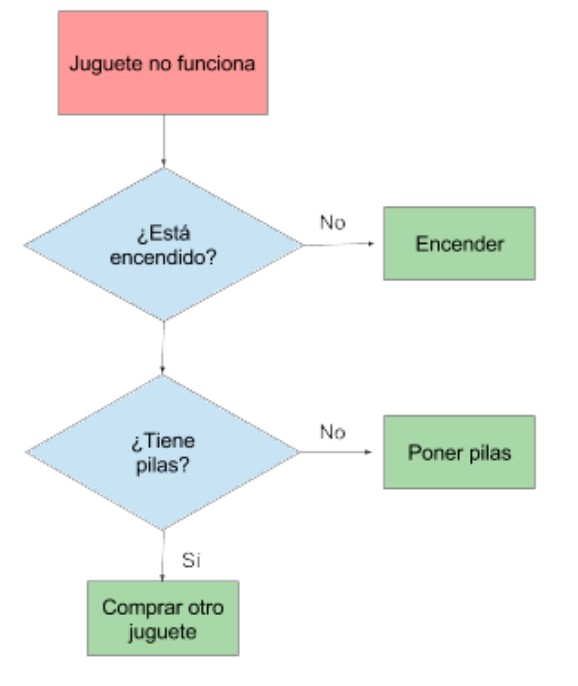
\includegraphics[scale=0.5]{algoritmo.jpg}
\caption{Diagrama de flujo de un algoritmo.}
\label{fig:universe}
\end{figure}

\end{defi}

\clearpage
\begin{defi}[Análisis a priori]
Acorde a la RAE, se puede definir la oraci\'on "a priori" c
omo  "‘por lo que precede’. En el ámbito de la filosofía, se emplea para referirse al conocimiento deductivo, esto es, al que se adquiere independientemente de la experiencia, yendo de las causas a los efectos y de lo universal a lo particular".
\\
En el analisis de algoritmos, se puede connotar que el analisis a priori sera aquel, el cual nos permita determinar la complejidad del mismo acorde a una notación, como lo pueden ser: Big O, $\Omega$, $\theta$.
\\
Para analizar dichos algoritmos es importante entender como funcionan los ordenes de complejidad dentro de los algoritmos, los cuales, podemos identificar en la siguiente tabla (Tabla 1: Orden de complejidad)
\\
\begin{table}[h!]
    \centering
    \begin{tabular}{|N|C|}
    \hline
        Orden & Nombre \\
    \hline
        O(1) & Constante \\
    \hline
        O($\log$ n) & Logarítmica \\
    \hline
        O(n) & lineal\\
    \hline
        O(n $\log$ n) & Casi lineal \\
    \hline
        O(n^{2}) & Cuadratica\\
    \hline
        O(n^{3}) & Cubica\\
    \hline
        O(a^{n}) & Exponencial\\
    \hline
    \end{tabular}
    \caption{Orden de complejidad}
    \label{tab:my_label}
\end{table}
\\
Asi mismo, se puede observar en la grafica siguiente, como se comportan cada uno de los ordenes de complejidad con relacion a su tasa de crecimiento,de donde el eje de las 'y' equivale al tiempo de ejecucion del algoritmo y en eje de las 'x' el contador, el cual idicara el orden de complejidad del algoritmo y a su vez sera delimitado por las cotas superior e inferior asintoticas, como se muestra en la siguiente figura (Figura 1: Tasa de crecimiento)

\begin{figure}[h!]
\centering
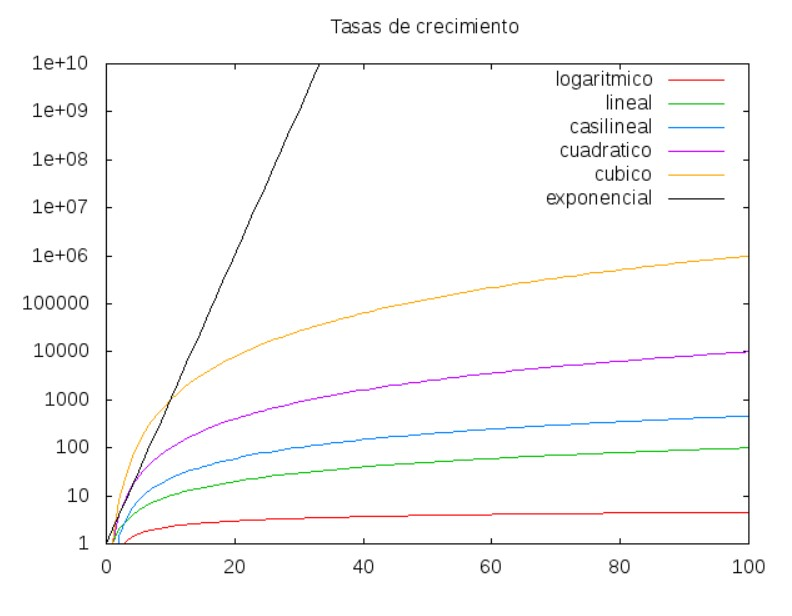
\includegraphics[scale=0.35]{orden de complejidad.jpg}
\caption{Tasa de crecimiento.}
\label{fig:tasa}
\end{figure}

\end{defi}
\clearpage
\\

\begin{defi}[Análisis a posteriori]
Acorde a la RAE, se define la oraci\'on "a posteriori" como  ‘por lo que viene después’. En el ámbito de la filosofía, se emplea para referirse al conocimiento inductivo, esto es, al que se adquiere a partir de la experiencia, ascendiendo de los efectos a las causas.
Así mismo, se connota que el an\'alisis a posteriori se recoge estadísticas de tiempo y espacio consumidas por el algoritmo mientras se ejecuta. 

\end{defi}
\begin{defi}[Notaci\'on O]
Es una herramienta que permite determinar la complejidad de un algoritmo determinando su rendimiento en cuanto a recursos y tiempo de ejecución, en pocas palabras identifica el peor caso donde el algoritmo llegue a su punto mas alto de exigencia.
\\
\\
Así mismo se acota de manera asintótica el crecimiento de un tiempo de ejecución a que este, dentro de factores constante por arriba y por abajo.
\\
\\
En la siguiente figura(Figura 3: Definicion Big O) se puede apreciar la cota superior asintotica, la cual esta resaltada en color azul. 
\begin{figure}[h!]
\centering
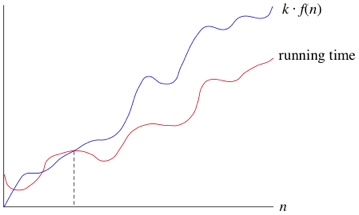
\includegraphics[scale=1.5]{big o.png}
\caption{Definici\'on Big O}
\label{fig:universe}
\end{figure}
\end{defi}
\clearpage
\begin{defi}[Notaci\'on $\Omega$]
Se usa la notación $\Omega$ para representar el limite asintótico inferior del tiempo de una funci\'on, esto quiere decir que, al contrario de la Notaci\'on O, se utiliza para calcularla complejidad de un algoritmo en su mejor caso.
\\
\\
En la siguiente grafica se puede apreciar lo que se denota como cota inferir asintotica, la cual esta resaltada en color azul.
\begin{figure}[h!]
\centering
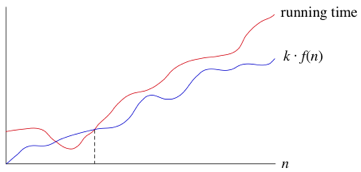
\includegraphics[scale=1.5]{big omega.png}
\caption{Definici\'on $\Omega$}
\label{fig:universe}
\end{figure}
\end{defi}

\begin{defi}[Notaci\'on $\Theta$]
Esta notaci\'on encierra a la funci\'on con un limite superior y un limite inferior. Se puede decir que se tiene una cota asintoticamente ajustada, esto por lo mencionado anteriormente ya que se ajusto el tiempo de ejecuci\'on (funci\'on) dentro del rango de una constante hacia arriba y hacia abajo. Esta notaci\'on se usa para calcular la complejidad de un algoritmo que no tiene mejor ni peor caso
\\
\\
En esta grafica se aprecia con mayor claridad ambas cotas, tanto la superior como la inferior, las cuales estan resaltadas en color azul. 
\begin{figure}[h!]
\centering
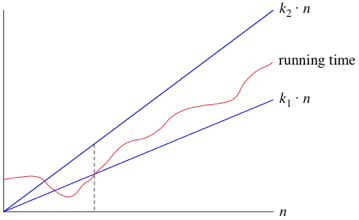
\includegraphics[scale=1.4]{big theta.png}
\caption{Definición $\Theta$}
\label{fig:universe}
\end{figure}
\end{defi}

\begin{algoritmo}[Fibonacci]
Este algoritmo busca calcular la sucesion de Fibonacci tanto en su forma recursiva, como en su forma iterativa, a las cuales se les aplicara el analsis a priori y el analisis a posteriri, a continuación en la Figure 6[Diagrama de flujo serie de Fibonnacci], se muestra el algoritmo de la serie de fibonnacci.

\begin{figure}[h!]
\centering
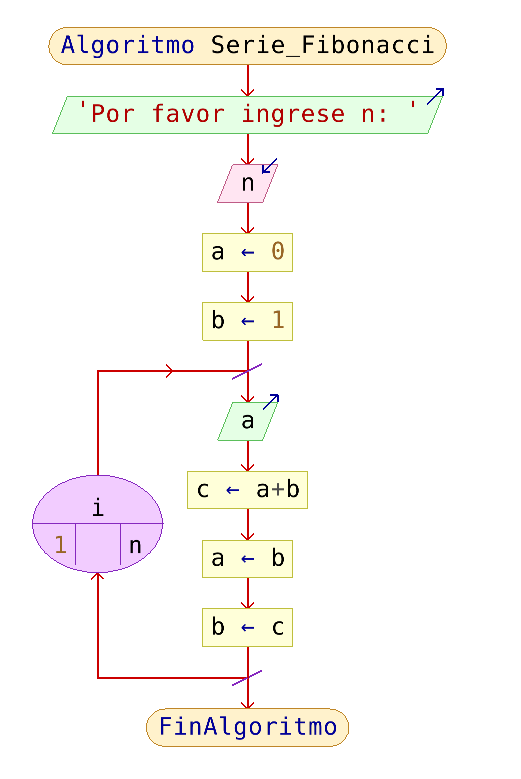
\includegraphics[scale=0.3]{fibonn.png}
\caption{Diagrama de flujo serie de Fibonnacci}
\label{fig:universe}
\end{figure}

\end{algoritmo}

\begin{algoritmo}[Numeros Perfectos]
Sabemos que un numero es perfecto si es igual a la suma de sus divisores menores; Es decir el numero 6 es un numero perfecto, porque 6=1+2+3. Se implemento ua funcion Perfecto(n), la cual dice si un numeor es perfecto o no, se le realizo el analisis a priori y a posteriori a dicha funcion, posteriormente se realizo otra funcion denominada MostrarPerfecto(n) la cual muestra los primeros n numeros perfecto, a esta funcion se le realizo el analisis a posteriori. 

\begin{figure}[h!]
\centering
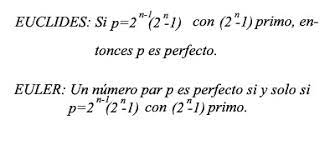
\includegraphics[scale=0.6]{perfectos.jpeg}
\caption{Ecuacion para calcular los números perfectos}
\label{fig:universe}
\end{figure}



\end{algoritmo}


 \section{Experimentaci\'on y Resultados}

\subsection{Ejercicio 1}
Realizar  el  análisis  a priori y  a posteriori para  el  problema  de la  suceción  de Fibonacci en su versión iterativa; y realizar su an álisis a posteriori en su versión recursiva.
\\
\\
Del siguiente algoritmo se calculo la complejidad y se obtuvo el resultado de Complejidad $\Theta$ (n)
\\
\\
Fibo(n)
\\
    a=0
\\
b=1
\\
for(i=0; i==n; i++)
\\
print(a)
\\
c=a+b
\\
a=b
\\
b=c
\\
\\
Al realizarle de hacerle el análisis a priori se llevo a cabo por bloques, en el cual se obtuvo una complejidad $\Theta$(1) y por el ciclo que tiene se obtiene una complejidad $\Theta$(n), concluyendo asi en la complejidad lineal.
\\
En este algoritmo el peor y el mejor caso son el mismo porque en ambos se tiene que calcular la sucesión de igual forma.
\newpage
\subsubsection{Caso general}
\subsubsection{Grafica del caso general}
\begin{figure}[h!]
\centering
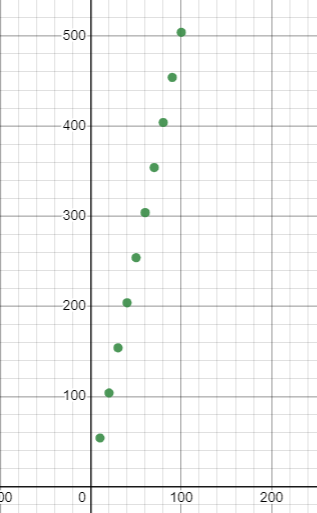
\includegraphics[scale=0.7]{graffibo.png}
\caption{Gráfica del caso general}
\label{fig:universe}
\end{figure}
\clearpage
\subsubsection{Tabla de valores}
Asi mismo, estas fueron las coordenadas para graficar el caso general, las cuales estan connotadas por N, quien es el n-simo termino de la sucesión, y ct que seria el contador de las veces que entra en ejecucion el codigo.
\\
\begin{center}
\begin{tabular}{|N|C|}
\hline
N & CT\\
\hline
10 & 54 \\
\hline
20 & 104\\
\hline
30 & 154\\
\hline
40 & 204\\
\hline
50 & 254\\
\hline
60 & 304\\
\hline
70 & 354\\
\hline
80 & 404\\
\hline
90 & 454\\
\hline
100 & 504\\
\hline
  
\end{tabular}
\end{center}
\subsubsection{Análisis}
En este caso como no existe una diferencia entre el mejor caso y el peor caso, se obtubo la sucesión de Fibonacci hasta n y la tabla grafica es la siguiente:
\begin{figure}[h!]
\centering
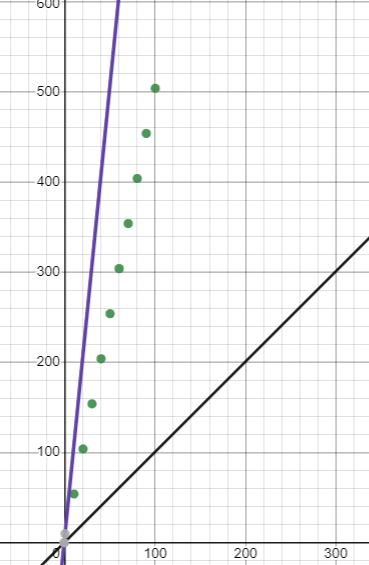
\includegraphics[scale=0.5]{graffiboas.png}
\caption{Gráfica}
\label{fig:universe}
\end{figure}
\clearpage
\subsection{Ejercicio 2}
Un número entero positivo es perfecto, si es igual a la suma de sus divisores menores. Por  ejemplo,  8  no  es  un  número  perfecto  ya  que  8 $\neq$ 1 + 2 + 4.
\\
Por otro lado,  6  si es un número perfecto, ya que 6 = 1 + 2 + 3. Implementar una función Perfecto(n) que decida si un número es perfecto o no. Realizar su análisis a priori y a posteriori para la función Perfecto(n). Haciendo uso de la función Perfecto(n), implementar una funcion MostrarPerfectos(n) que muestre los n primeros números perfectos. Realizar su análisis a posteriori para la función MostrarPerfectos(n). ¿Cúantos números perfectos logro generar en su computadora?
\\
Del siguiente algoritmo se calculo la complejidad y se obtuvo el resultado de Complejidad $\Theta$ {(n^2)}
\\
\\
Perfecto(n)
\\
divisores 
\\
suma
\\
salida
\\
for (i=1; i==n; i++)
\\
if (n%i) == 0 
\\
divisores.apend(i)
\\
for (i; i==divisores; i++)
\\
suma=suma+i
\\
if suma == n 
\\
numerosperfectos 
\\
salida
\\
else 
\\
salida
\\
return print(salida)
\\
\\

Al realizarle el análisis a posteriori se llevo a cabo por bloques, en el cual se obtuvo una complejidad $\Theta$(1) y por el ciclo que tiene se obtiene una complejidad $\Theta$(n), concluyendo asi en la complejidad es cuadratica. 


\clearpage

\newpage
\subsubsection{Caso general}
\\
En este caso la computadora utilizada para calcular los números perfectos solo pudo encontrar el quinto numero perfecto, el cual es: '33,550,336', y el tiempo de ejecucion fue de aproximdamente 9 hrs.  
\\
\\
Esto permite concluir que el algoritmo es cuadratico, ya que entre mas numeros de la series se quieran encontrar mayor sera la cantidad de tiempo que tarde en encontrarlos. Obviamente esto tambiem es completamente dependiente del poder de computo del cual se disponga en el momento de ejecutar el algoritmo. Entre mas y mejor poder de computo el algoritmo se tomara menor tiempo, pero ello no queire decir que su dificultad se reducira, esta se mantendra, es decir que seguira siendo cuadratica.
\\
Resumiendo el algoritmo siempre sera de complejiad cuadratica y entre mayor cantidad de numeros perfectos se quieran encontrar mucho mayor sera el tiempo que tarde en encontrarlos.

\clearpage
\subsubsection{Grafica del caso general}
Aqui, se determina que la complejidad del algoritmo en su caso general, es cuadratica.
\begin{figure}[h!]
\centering
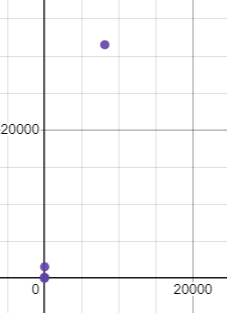
\includegraphics[scale=0.7]{grafper.png}
\caption{Gráfica del caso general}
\label{fig:universe}
\end{figure}

\begin{figure}[h!]
\centering
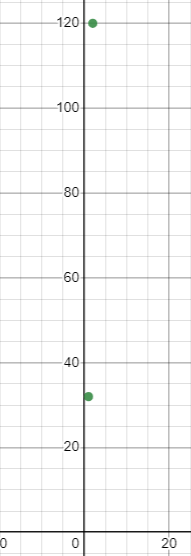
\includegraphics[scale=0.7]{Perf1.png}
\caption{Gráfica del caso general donde se aprecia con un zoom los primeros 2 puntos}
\label{fig:universe}
\end{figure}

\begin{figure}[h!]
\centering
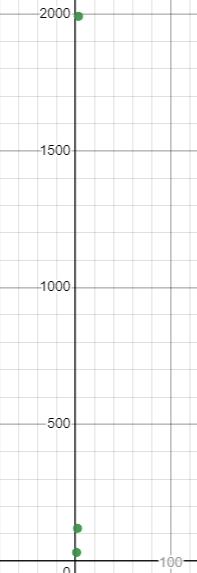
\includegraphics[scale=0.7]{perf2.png}
\caption{Gráfica del caso general donde se aprecia con un zoom los primeros 3 puntos}
\label{fig:universe}
\end{figure}

\begin{figure}[h!]
\centering
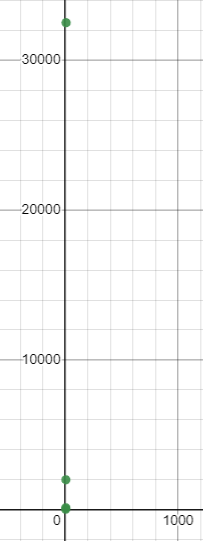
\includegraphics[scale=0.7]{perf3.png}
\caption{Gráfica del caso general donde se aprecia con un zoom los primeros 4 puntos}
\label{fig:universe}
\end{figure}
\subsubsection{Tabla de valores Perfecto}
Asi mismo, estas fueron las coordenadas para graficar el caso general, las cuales estan connotadas por N, quien es la cantidad de numeros perfectos encontrados, y ct que seria el contador de las veces que entra en ejecucion el codigo, asi mismo, se pueden ver en las Figuras 11, 12 y 13, como se va comportando la recta.
\\
\begin{center}
\begin{tabular}{|N|C|}
\hline
N & CT\\
\hline
1 &  32\\
\hline
2 & 120\\
\hline
3 & 1992\\
\hline
4 & 32520\\
\hline  
\end{tabular}
\end{center}


\clearpage

\section{Conclusiones}
Conclusión Martinez Lopez Sebastian:\\
Durante el desarrollo de esta practica la principal dificultad que se presento fue al momento de realizar y cualcular la complejidad de los algoritmos, mas precisamente al momento de realizar el analisis a priori de cada una de las funciones, una vez resuelto esto el resto fue mas sencillo, ya que nos permite entender de mejor forma como funciona el mismo y como se comporta, a su vez nos da una idea de cuanto tiempo tarda el agoritmo en realizar todas las tarea.
 
\begin{figure}[h!]
\centering
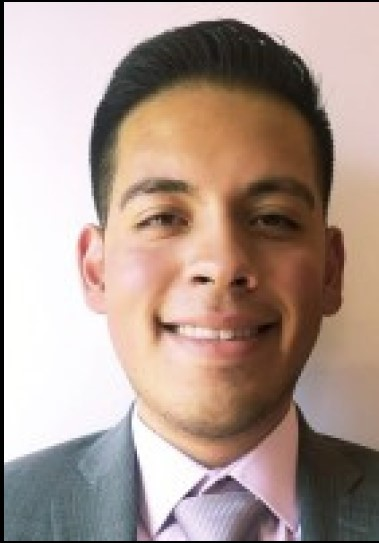
\includegraphics[scale=0.3]{seb1.jpg}
\label{fig:universe}
\end{figure}
\\

Conclusión Ramirez Resendiz Luis Roque:\\
Durante el desarrollo de esta practica se obserba que un solo algoritmo puede cambiar de complejidad dependiendo del caso en el que se encuentre y de igual manera que un algortmo puede tener la misma complejidad tanto en su mejor caso como en el peor. De esta manera se puede valorar y realizar un análisis a fondo sobre dicho algoritmo, otorgando la oportunidad de compararlo con otros algoritmos que resuelvan el mismo problema de esta manera asi poder implementar el algoritmo que mas convenga, obviamente basándose en las necesidades o el para que se requiere el algoritmo. De la misma forma se comprobo que cuando un algoritmo tiene una cierta complejidad, esta no va a cambiar auqnue exista un mejor poder de computo, ya que como se observo en el algoritmo de MostrarPerfectos en donde la computadora en cuestion solo logro calcular hasta el quito termio y el tiempo que le tomo fue considerablemente mayor al que le tomo cacular el cuarto termino. 
\begin{figure}[h!]
\centering

\includegraphics[scale=0.5]{luis1.jpg}

\label{fig:universe}
\end{figure}
\newpage

\section{Bibliograf\'ia}
\\
Notación big O. (s/f). Pablocianes.com. Recuperado el 7 de septiembre de 2022, de https://pablocianes.com/notacion-big-o/
\\
\\
Notación Omega grande (Big-Ω). (s/f). Khan Academy. Recuperado el 7 de septiembre de 2022, de https://es.khanacademy.org/computing/computer-science/algorithms/asymptotic-notation/a/big-big-omega-notation
\\
\\
Notación θ grande (Big-θ). (s/f). Khan Academy. Recuperado el 7 de septiembre de 2022, de https://es.khanacademy.org/computing/computer-science/algorithms/asymptotic-notation/a/big-big-theta-notation
\\
\\
(S/f). Rae.es. Recuperado el 25 de octubre de 2022, de https://www.rae.es/dpd/a%20priori
\\
\\
(S/f-a). Rae.es. Recuperado el 25 de septiembre de 2022, de https://dle.rae.es/algoritmo
\\
\\
(S/f-b). Rae.es. Recuperado el 25 de septiembre de 2022, de https://www.rae.es/dpd/a%20posteriori
\\
\\
(S/f-c). Rae.es. Recuperado el 25 de septiembre de 2022, de https://www.rae.es/dpd/anterior
\\
\\
BBC News Mundo. (2020, diciembre 6). Por qué el 6 es un número perfecto pero el 7 definitivamente no. BBC. https://www.bbc.com/mundo/noticias-55179824
\\
\\
¿Cómo calcular el Algoritmo de Fibonacci en Scala? (2022, febrero 15). KeepCoding Tech School. https://keepcoding.io/blog/que-es-el-algoritmo-de-fibonacci/

\medskip



\end{document}
